%% LyX 2.1.3 created this file.  For more info, see http://www.lyx.org/.
%% Do not edit unless you really know what you are doing.
\documentclass[oneside]{amsart}
\usepackage[latin9]{inputenc}
\setlength{\parskip}{\medskipamount}
\setlength{\parindent}{0pt}
\usepackage{float}
\usepackage{mathtools}
\usepackage{amsthm}
\usepackage{amsbsy}
\usepackage{amstext}
\usepackage{amssymb}
\usepackage{cancel}
\usepackage{stmaryrd}
\usepackage{graphicx}
\usepackage{esint}

\makeatletter
%%%%%%%%%%%%%%%%%%%%%%%%%%%%%% Textclass specific LaTeX commands.
\numberwithin{equation}{section}
\numberwithin{figure}{section}
  \theoremstyle{plain}
  \newtheorem*{cor*}{\protect\corollaryname}

%%%%%%%%%%%%%%%%%%%%%%%%%%%%%% User specified LaTeX commands.

%
\usepackage{amsfonts}
%\usepackage{mathabx}
\usepackage{nopageno}%%%  The following few lines affect the margin sizes. 
\usepackage{bm}
\addtolength{\topmargin}{-.5in}
\setlength{\textwidth}{6in}       
\setlength{\oddsidemargin}{.25in}              
\setlength{\evensidemargin}{.25in}         
  
\setlength{\textheight}{9in}
\renewcommand{\baselinestretch}{1}
\reversemarginpar   
%
%

\makeatother

\usepackage{listings}
  \providecommand{\corollaryname}{Corollary}
\renewcommand{\lstlistingname}{Listing}

\begin{document}

\title{ESI 6420 Homework 2 Solutions}


\author{Maksim Levental}


\date{\today}

\maketitle
Time spent: too much but time well spent is never wasted.

Collaborators: Chris Gianelli.
\begin{enumerate}
\item [1.1] The model for this SVM is similar to the typical SVM model
except with some binary integer variables and constraints on those
variables: the standard SVM (with data $\mathbf{x}_{i}\in\mathbb{R}^{n}$
for $i=1,\dots,k$ and class assignments $y_{i}\in\left\{ -1,1\right\} $)
is 
\begin{align*}
\min_{\boldsymbol{\alpha}\in\mathbb{R}^{n}} & \left\Vert \boldsymbol{\alpha}\right\Vert \\
\text{s.t.} & y_{i}\left(\boldsymbol{\alpha}\cdot\mathbf{x}_{i}-\beta\right)\geq1\,\forall i\in\left\{ 1,\dots,k\right\} 
\end{align*}
The ``incomplete SVM'' introduces two new binary integer variables
$\mathbf{b}\in\left\{ 0,1\right\} ^{k}$ and $\mathbf{p}\in\left\{ 0,1\right\} ^{n}$.
They are incorporated as such: \textbf{$b_{i}$ }determines whether
constraint $y_{i}\left(\boldsymbol{\alpha}\cdot\mathbf{x}_{i}-\beta\right)\geq1\iff y_{i}\left(\boldsymbol{\alpha}\cdot\mathbf{x}_{i}-\beta\right)-1\geq0$
is active. This is effected by multipltying the constraint by $b_{i}:$
\[
b_{i}\left(y_{i}\left(\boldsymbol{\alpha}\cdot\mathbf{x}_{i}-\beta\right)-1\right)\geq0
\]
If $b_{i}=1$ then the constraint is left as is and if $b_{i}=0$
then the constraint is automatically satisfied as $0\geq0$. Then
the constraint on how many constraint equations can be active is effected
by using 0-norm:
\[
\left\Vert \mathbf{b}\right\Vert _{0}\geq100-K
\]
The sparsity of $\boldsymbol{\alpha}$ is controlled by $p_{i}$ in
the same way. The margin constraints transform further into 
\[
b_{i}\left(y_{i}\left(\sum_{i=1}^{n}p_{i}\alpha_{i}x_{i}-\beta\right)-1\right)\geq0
\]
and maximum ``density'' (as opposed to sparsity) is controlled by
\[
\left\Vert \mathbf{p}\right\Vert _{0}\leq M
\]
Therefore the model is for some $K,M$ 
\begin{align*}
\min_{\underset{\underset{,\mathbf{p}\in\left\{ 0,1\right\} ^{n}}{\mathbf{b}\in\left\{ 0,1\right\} ^{k}}}{\boldsymbol{\alpha}\in\mathbb{R}^{n}}} & \left\Vert \boldsymbol{\alpha}\right\Vert \\
\text{s.t.} & b_{i}\left(y_{i}\left(\sum_{i=1}^{n}p_{i}\alpha_{i}x_{i}-\beta\right)-1\right)\geq0\,\forall i\in\left\{ 1,\dots,k\right\} \\
\left\Vert \mathbf{b}\right\Vert _{0} & \geq100-K\\
\left\Vert \mathbf{p}\right\Vert _{0} & \leq M
\end{align*}

\item [1.2] I wrote AMPL code instead of GAMS code because AMPL $\gg$
GAMS.
\begin{lstlisting}
set cnts := 1 .. 20;
set dps := 1 .. 100; 
param x{dps,cnts};
param y{dps};
param omit_points;
param nz_a;
var afa {cnts};
var b {dps} binary integer;
var p {cnts} binary integer;
var bta;
minimize obj: sum{c in cnts} alpha[c]*alpha[c];
s.t. mgn{d in dps}: b[d]*(y[d]*((sum{c in cnts} p[c]*afa[c]*x[d,c])-bta)-1)>=0;
s.t. cstnt_msk:  sum{d in dps} b[d] >= 100 - omit_points;
s.t. non_z_a: sum{c in cnts} p[c] <= nz_a; 

data;

param y := <snip>
param x := <snip>

script;

set omitted_data;
set max_nonzero_alpha;
param om{omitted_data};
param ma{max_nonzero_alpha};
let omitted_data := 4 .. 16 by 2;
let max_nonzero_alpha := 3 .. 6;
for {o in omitted_data} {
	for {m in max_nonzero_alpha} {
		let omit_points := o;
		let nz_a := m;
		option solver couenne;
		solve;
		display sqrt(sum{c in cnts} afa[c]*afa[c]);
		display afa;
		display b;
		display o;
		display m;
		display p;
		display beta;
	}
}
\end{lstlisting}

\item [1.3]Pictures
\begin{figure}[H]
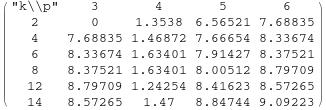
\includegraphics[scale=0.75]{mu_table.jpeg}\protect\caption{$\mu\left(k,p\right)$ table}


\end{figure}
\begin{figure}[H]
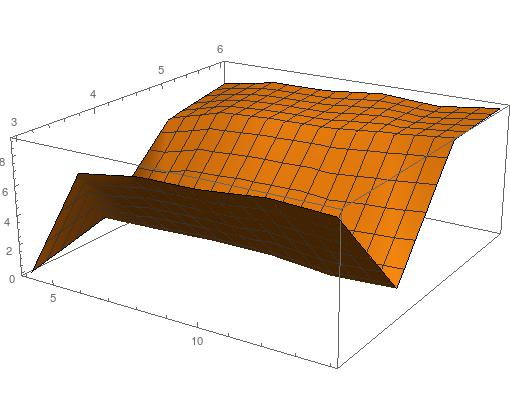
\includegraphics[scale=0.5]{mu_pic.jpeg}\protect\caption{$\mu\left(k,p\right)$ picture}
\end{figure}

\item [2.1]Claim: For $A\in\mathbb{R}^{m\times n}$, $B\in\mathbb{R}^{k\times n}$
, if for all $x$ it's the case that $Ax=0$ implies $Bx=0$ then
$B=CA$ for some $C\in\mathbb{R}^{k\times m}$.

\begin{proof}
Assume without loss of generality that and $k\leq m$. Suppose $Ax=0\Rightarrow Bx=0$.
This is equivalent to $\text{null}\left(A\right)\subset\text{null}\left(B\right)$.
By the fundamental theorem of Linear Algebra and the fact that $\text{row}\left(A\right)\subset\mathbb{R}^{n}$
and $\text{row}\left(B\right)\subset\mathbb{R}^{n}$ we have that
$\text{null}\left(A\right)\cup\text{row}\left(A\right)=\text{null}\left(B\right)\cup\text{row}\left(B\right)=\mathbb{R}^{n}$
and hence 
\begin{align*}
\text{null}\left(A\right) & \subset\text{null}\left(B\right)\\
 & \iff\\
\overline{\text{null}\left(A\right)} & \subset\overline{\text{null}\left(B\right)}\\
 & \iff\\
\text{row}\left(B\right) & \subset\text{row}\left(A\right)
\end{align*}
Therefore for all $i=1,\dots,k$ there exist $c_{i}\in\mathbb{R}^{m}$
such that
\[
A^{T}c_{i}=b_{i}^{T}
\]
where $b_{i}^{T}=\left(B^{T}\right)_{i}$ the $i$th row of $B$.
Collecting all of the $c_{i}$ into a matrix $C^{T}$ we get that
\[
A^{T}C^{T}=B^{T}
\]
or 
\[
CA=B
\]

\end{proof}
\item [2.2]Claim: For $\left\{ v_{1},\dots,v_{m}\right\} \subset\mathbb{R}^{n}$
and $m\geq n+2$ there exist $\boldsymbol{\alpha}=\left(\alpha_{1},\dots,\alpha_{m}\right)\neq\mathbf{0}$
such that 
\[
\sum_{i=1}^{m}\alpha_{i}v_{i}=0
\]
and
\[
\sum_{i=1}^{m}\alpha_{i}=0
\]


\begin{proof}
Assume $m\geq n+2$. Let 
\[
w_{i}=\begin{pmatrix}v_{i}\\
1
\end{pmatrix}
\]
Note that $w_{i}\in\mathbb{R}^{\left(n+1\right)}$. Since $m\geq n+2$
it's the case that $m>n+1$ and hence $\left\{ w_{1},\dots,w_{m}\right\} $
is linearly dependent (since the maximal number of linearly independent
vectors in $\mathbb{R}^{\left(n+1\right)}$ is $n+1$). Therefore,
with $W=\left(w_{1},w_{2},\dots,w_{m}\right)$ it must be case that
there exists $\boldsymbol{\alpha}\in\mathbb{R}^{m}$ such that 
\begin{align*}
W\boldsymbol{\alpha} & =\begin{pmatrix}v_{1} & \cdots & v_{m}\\
1 & \cdots & 1
\end{pmatrix}\begin{pmatrix}\alpha_{1}\\
\vdots\\
\alpha_{m}
\end{pmatrix}\\
 & =\begin{pmatrix}\sum_{i=1}^{m}\alpha_{i}v_{i}\\
\sum_{i=1}^{m}\alpha_{i}
\end{pmatrix}\\
 & =\mathbf{0}
\end{align*}

\end{proof}
\item [2.3]Claim: For $A:U\rightarrow V$ and $B:V\rightarrow W$ linear
maps
\[
\dim\left(R\left[A\right]\cap\ker\left[B\right]\right)=\dim\left(R\left[A\right]\right)-\dim\left(R\left[BA\right]\right)=\dim\left(\ker\left[BA\right]\right)-\dim\left(\ker\left[A\right]\right)
\]
\begin{align*}
\dim\left(R\left[BA\right]\right) & =\dim\left(R\left[A\right]\right)-\dim\left(R\left[A\right]\cap\ker\left[B\right]\right)\\
\dim\left(R\left[A\right]\right)+\dim\left(\ker\left[A\right]\right) & =\dim\left(\ker\left[BA\right]\right)+\dim\left(R\left[BA\right]\right)
\end{align*}
where $R\left[X\right]$ is the column-space of $X$.

\begin{proof}
Let $u,v,w$ be the dimensions of $U,V,W$ respectively. Since $BA:U\rightarrow W$
the rank-nullity theorem states that 
\[
\text{rank}\left(A\right)+\text{nullity}\left(A\right)=u=\text{rank}\left(BA\right)+\text{nullity}\left(BA\right)
\]
and since $\text{rank}\left(X\right)=\dim\left(R\left[X\right]\right)$
and $\text{nullity}\left(X\right)=\dim\left(\ker\left[X\right]\right)$
it's the case that 
\[
\dim\left(R\left[A\right]\right)+\dim\left(\ker\left[A\right]\right)=\dim\left(\ker\left[BA\right]\right)+\dim\left(R\left[BA\right]\right)
\]
or
\[
\dim\left(R\left[A\right]\right)-\dim\left(R\left[BA\right]\right)=\dim\left(\ker\left[BA\right]\right)-\dim\left(\ker\left[A\right]\right)
\]
Now let $\left\{ u_{1},\dots,u_{k}\right\} $ be a basis for $R\left[A\right]\cap\ker\left[B\right]$.
The set $\left\{ u_{1},\dots,u_{k}\right\} $ is linearly independent
in $R\left[A\right]$ and hence can be extended to a basis: let $\left\{ u_{1},\dots,u_{k},v_{1},\dots,v_{n}\right\} $
be a basis for $R\left[A\right]$. Finally let $\left\{ y_{1},\dots,y_{m}\right\} $
be a basis for $R\left[BA\right]$ and pick an arbitrary $y_{i}$.
By definition there exists $x_{i}$ such that 
\[
BAx_{i}=y_{i}
\]
But $Ax_{i}$ is in $R\left[A\right]$ and therefore there exist $\left\{ \alpha_{1},\dots,\alpha_{k},\beta_{1},\dots,\beta_{n}\right\} $
such that 
\[
Ax_{i}=\sum_{i=1}^{k}\alpha_{i}u_{i}+\sum_{i=1}^{n}\beta_{i}v_{i}
\]
But 
\[
y_{i}=B\left(Ax_{i}\right)=B\left(\sum_{i=1}^{k}\alpha_{i}u_{i}+\sum_{i=1}^{n}\beta_{i}v_{i}\right)=\sum_{i=1}^{k}\alpha_{i}Bu_{i}+B\left(\sum_{i=1}^{n}\beta_{i}v_{i}\right)
\]
and by $\left\{ u_{i}\right\} $ being a basis for $\ker\left[B\right]$
\[
y_{i}=\cancel{\sum_{i=1}^{k}\alpha_{i}Bu_{i}}+B\left(\sum_{i=1}^{n}\beta_{i}v_{i}\right)=\sum_{i=1}^{n}\beta_{i}Bv_{i}=\sum_{i=1}^{n}\beta_{i}w_{i}
\]
where $w_{i}\coloneqq Bv_{i}$. Therefore 
\[
R\left[BA\right]=\text{span}\left(\left\{ y_{1},\dots,y_{m}\right\} \right)=\text{span}\left(\left\{ w_{1},\dots,w_{n}\right\} \right)
\]
but note that $\left\{ w_{1},\dots,w_{n}\right\} $ is linearly independent:
if there existed $\left\{ \gamma_{1},\dots,\gamma_{n}\right\} $ such
that $\sum_{i=1}^{n}\gamma_{i}w_{i}=0$ then 
\[
\sum_{i=1}^{n}\gamma_{i}w_{i}=\sum_{i=1}^{n}\gamma_{i}Bv_{i}=B\left(\sum_{i=1}^{n}\gamma_{i}v_{i}\right)=0
\]
and $\left\{ v_{1},\dots,v_{n}\right\} $ were defined to be linearly
independent of $\ker\left[B\right]$ (and hence no vector in their
span could be in $\ker\left[B\right]$). Hence (finally) 
\begin{align*}
\dim\left(R\left[BA\right]\right) & =\dim\left(\text{span}\left(\left\{ y_{1},\dots,y_{m}\right\} \right)\right)\\
 & =\dim\left(\text{span}\left(\left\{ w_{1},\dots,w_{n}\right\} \right)\right)\\
 & =\dim\left(\left\{ u_{1},\dots,u_{k},v_{1},\dots,v_{n}\right\} \backslash\left\{ u_{1},\dots,u_{k}\right\} \right)
\end{align*}
and $\left\{ u_{1},\dots,u_{k}\right\} $ and $\left\{ v_{1},\dots,v_{n}\right\} $
are linearly independent 
\begin{align*}
\dim\left(R\left[BA\right]\right) & =\dim\left(\left\{ u_{1},\dots,u_{k},v_{1},\dots,v_{n}\right\} \backslash\left\{ u_{1},\dots,u_{k}\right\} \right)\\
 & =\dim\left(\left\{ u_{1},\dots,u_{k},v_{1},\dots,v_{n}\right\} \right)-\dim\left(\left\{ u_{1},\dots,u_{k}\right\} \right)\\
 & =\dim\left(R\left[A\right]\right)-\dim\left(R\left[A\right]\cap\ker\left[B\right]\right)
\end{align*}

\begin{cor*}
For $D$ a linear operator
\[
\dim\left(\ker\left[D^{n+1}\right]\right)=\dim\left(\ker\left[D\right]\right)+\sum_{j=1}^{n}\dim\left(R\left[D^{k}\right]\cap\ker\left[D\right]\right)
\]
\end{cor*}
\begin{proof}
By induction on $n$. Let $n=1$ and by the (manipulated above) result
with $A=B=D$

\[
\dim\left(R\left[D\right]\cap\ker\left[D\right]\right)+\dim\left(\ker\left[D\right]\right)=\dim\left(\ker\left[DD\right]\right)
\]
or 
\[
\dim\left(\ker\left[D^{1+1}\right]\right)=\dim\left(\ker\left[D\right]\right)+\sum_{j=1}^{1}\dim\left(R\left[D^{k}\right]\cap\ker\left[D\right]\right)
\]
Assume $n>1$. Then by applying the above result again with $B=D^{n}$
and $A=D$, and applying the induction hypothesis 
\begin{align*}
\dim\left(\ker\left[D^{n+1}\right]\right) & =\dim\left(\ker\left[D^{1}D^{n}\right]\right)\\
 & =\dim\left(R\left[D^{n}\right]\cap\ker\left[D\right]\right)+\dim\left(\ker\left[D\right]\right)\\
 & =\dim\left(R\left[D^{n}\right]\cap\ker\left[D\right]\right)+\dim\left(\ker\left[D\right]\right)\\
 & +\sum_{j=1}^{n-1}\dim\left(R\left[D^{k}\right]\cap\ker\left[D\right]\right)\\
 & =\dim\left(\ker\left[D\right]\right)+\sum_{j=1}^{n}\dim\left(R\left[D^{k}\right]\cap\ker\left[D\right]\right)
\end{align*}

\end{proof}
\end{proof}
\item [2.5]Claim: For $V$ and $n$-dimensional real vector space and $U,W$
$m$-dimensional subspaces of $V$, if there exists $u^{'}\in U\backslash\left\{ 0\right\} $
such that $u^{'}\perp W$ then there exists $w\in W\backslash\left\{ 0\right\} $
such that $w\perp U\backslash\left\{ 0\right\} $.

\begin{proof}
Suppose not. Then there does not exist $w$ such that $w\cdot u=0$
for all $u\in U$. That means for every $w$ there exists $u$ such
that $u\cdot w\neq0$. Fix a basis $\left\{ w_{1},\dots,w_{m}\right\} $
for $W$. Then there exist $\left\{ u_{1},\dots,u_{m}\right\} $ such
that $w_{i}\cdot u_{i}\neq0$ for all $i=1,\dots,m$. Note that $\left\{ u_{1},\dots,u_{m}\right\} $
can be chosen such that they are necessarily linearly dependent. Why?
Let 
\[
\upsilon_{i}=u_{i}-\left(u_{i}\cdot u^{'}\right)\frac{u^{'}}{\left\Vert u^{'}\right\Vert _{2}}
\]
and then $u^{'}\perp\upsilon_{i}$ for all $i=1,\dots,m$ (but $w_{i}\cdot\upsilon_{i}$
is still non-zero) and hence $\left\{ u^{'},\upsilon_{1},\dots,\upsilon_{m}\right\} $
would be a linearly independent set of $m+1$ vectors in $U$ an $m$-dimensional
vector space. So there exist $\alpha_{i}$ such that 
\[
\sum_{i=1}^{m}\alpha_{i}\upsilon_{i}=0
\]
or
\[
\upsilon_{1}=-\sum_{i=2}^{m}\alpha_{i}\upsilon_{i}
\]
Then 
\[
\sum_{i=1}^{n}\left(w_{i}\cdot\upsilon_{i}\right)w_{i}=\left(w_{1}\cdot\left(-\sum_{i=2}^{m}\alpha_{i}\upsilon_{i}\right)\right)w_{1}+\sum_{i=2}^{n}\left(w_{i}\cdot\upsilon_{i}\right)w_{i}
\]
\[
\left(w_{1}\upsilon_{1}\right)w_{1}+\left(w_{2}\upsilon_{2}\right)w_{2}=\left(w_{1}\upsilon_{1}\right)w_{1}+\left(w_{2}\left(c\upsilon_{1}\right)\right)w_{2}=\left(w_{1}\upsilon_{1}\right)w_{1}+\left(w_{2}\left(c\upsilon_{1}\right)\right)w_{2}
\]


And I have no clue..................
\end{proof}
\item [3.1]Claim: $\left\langle \left\langle I\right\rangle \right\rangle \geq1$
for all matrix norms $\left\langle \left\langle \cdot\right\rangle \right\rangle $. 

\begin{proof}
Since $II=I$ we have that 
\[
\left\langle \left\langle I\right\rangle \right\rangle =\left\langle \left\langle II\right\rangle \right\rangle \leq\left\langle \left\langle I\right\rangle \right\rangle \left\langle \left\langle I\right\rangle \right\rangle 
\]
cancelling $\left\langle \left\langle I\right\rangle \right\rangle $
from both sides of the inequality we have that 
\[
1\leq\left\langle \left\langle I\right\rangle \right\rangle 
\]

\end{proof}
\item [3.2]Claim: The Frobenius norm 
\[
\left\langle \left\langle A\right\rangle \right\rangle _{F}=\sqrt{\text{tr}\left(A^{T}A\right)}=\sqrt{\sum_{i}\sum_{j}\left|a_{ij}\right|^{2}}
\]
is a matrix norm.

\begin{proof}
It is positively homogenous, subadditive, and positive definite because
it is equivalent to the Euclidean norm on $\mathbb{R}^{n^{2}}$. Further
it satisfies ``submultiplicativity'': first note that for $A,B$
\[
\left(AB\right)_{ij}=\sum_{k}a_{ik}b_{kj}
\]
Therefore 
\begin{align*}
\left\langle \left\langle AB\right\rangle \right\rangle _{F} & =\sqrt{\sum_{i}\sum_{j}\left(\left(AB\right)_{ij}\right)^{2}}\\
 & =\sqrt{\sum_{i}\sum_{j}\left(\left|\sum_{k}a_{ik}b_{kj}\right|\right)^{2}}
\end{align*}
now by Cauchy-Schwarz
\begin{align*}
\left\langle \left\langle AB\right\rangle \right\rangle _{F} & =\sqrt{\sum_{i}\sum_{j}\left(\left(AB\right)_{ij}\right)^{2}}\\
 & =\sqrt{\sum_{i}\sum_{j}\left(\left|\sum_{k}a_{ik}b_{kj}\right|\right)^{2}}\\
 & \leq\sqrt{\sum_{i}\sum_{j}\left(\sum_{k}\left|a_{ik}\right|^{2}\sum_{k}\left|b_{kj}\right|^{2}\right)}\\
 & =\sqrt{\left(\sum_{i}\sum_{k}\left|a_{ik}\right|^{2}\right)\left(\sum_{j}\sum_{k}\left|b_{kj}\right|^{2}\right)}\\
 & =\left\langle \left\langle A\right\rangle \right\rangle _{F}\left\langle \left\langle B\right\rangle \right\rangle _{F}
\end{align*}

\end{proof}
\item [3.3]Let the induced matrix $p$-norm be
\[
\left\langle \left\langle A\right\rangle \right\rangle _{p}=\sup_{x\in\mathbb{R}^{n}\backslash\left\{ 0\right\} }\frac{\left\Vert Ax\right\Vert _{p}}{\left\Vert x\right\Vert _{p}}
\]


\begin{enumerate}
\item Claim: The induced matrix $p$-norm is equivalent to
\[
\left\langle \left\langle A\right\rangle \right\rangle _{p}=\sup_{x\in\mathbb{R}^{n},\left\Vert x\right\Vert _{p}=1}\left\Vert Ax\right\Vert _{p}
\]


\begin{proof}
Let $y$ be such that 
\[
y=\text{argmax}\left(\frac{\left\Vert Ax\right\Vert _{p}}{\left\Vert x\right\Vert _{p}}\right)
\]
Then 
\[
\left\langle \left\langle A\right\rangle \right\rangle _{p}=\frac{\left\Vert Ay\right\Vert _{p}}{\left\Vert y\right\Vert _{p}}
\]
Let $z\in\mathbb{R}^{n},c\in\mathbb{R}$ be such that $cz=y$ and
$\left\Vert z\right\Vert _{p}=1$. Then 
\begin{align*}
\frac{\left\Vert Ay\right\Vert _{p}}{\left\Vert y\right\Vert _{p}} & =\frac{\left\Vert A\left(cz\right)\right\Vert _{p}}{\left\Vert cz\right\Vert _{p}}
\end{align*}
Then by linearity of matrix multiplication and the $p$-norm
\begin{align*}
\frac{\left\Vert c\right\Vert _{p}\left\Vert Az\right\Vert _{p}}{\left\Vert c\right\Vert _{p}\left\Vert z\right\Vert _{p}} & =\frac{\left\Vert Az\right\Vert _{p}}{\left\Vert z\right\Vert _{p}}\\
 & =\left\Vert Az\right\Vert _{p}
\end{align*}
Now suppose that there were some $z'$ such that $\left\Vert z'\right\Vert _{p}=1$
and $\left\Vert Az'\right\Vert _{p}>\left\Vert Az\right\Vert _{p}$.
Then 
\begin{align*}
\left\Vert Az'\right\Vert _{p}>\left\Vert Az\right\Vert _{p} & =\frac{\left\Vert Az\right\Vert _{p}}{\left\Vert z\right\Vert _{p}}=\frac{\left\Vert A\frac{y}{c}\right\Vert _{p}}{\left\Vert \frac{y}{c}\right\Vert _{p}}=\frac{\left\Vert \frac{1}{c}\right\Vert _{p}\left\Vert Ay\right\Vert _{p}}{\left\Vert \frac{1}{c}\right\Vert _{p}\left\Vert y\right\Vert _{p}}=\frac{\left\Vert Ay\right\Vert _{p}}{\left\Vert y\right\Vert _{p}}
\end{align*}
which is a contradiction (since $y$ was defined to the argmax of
$\left\Vert Ax\right\Vert _{p}/\left\Vert x\right\Vert _{p}$). Hence
it sufficies to define 
\[
\left\langle \left\langle A\right\rangle \right\rangle _{p}=\sup_{x\in\mathbb{R}^{n},\left\Vert x\right\Vert _{p}=1}\left\Vert Ax\right\Vert _{p}
\]

\end{proof}
\item Claim: the induced matrix $p$-norm is a legitimate matrix norm.

\begin{proof}
Using the equivalent definition from part (a) we prove
\begin{enumerate}
\item Positive homogenous: let $c\in\mathbb{R}$ and then by the homogeneity
of the $p$-norm 
\begin{align*}
\left\langle \left\langle cA\right\rangle \right\rangle _{p} & =\sup_{x\in\mathbb{R}^{n},\left\Vert x\right\Vert _{p}=1}\left\Vert \left(cA\right)x\right\Vert _{p}\\
 & =\sup_{x\in\mathbb{R}^{n},\left\Vert x\right\Vert _{p}=1}\left|c\right|\left\Vert Ax\right\Vert _{p}\\
 & =\left|c\right|\left(\sup_{x\in\mathbb{R}^{n},\left\Vert x\right\Vert _{p}=1}\left\Vert Ax\right\Vert _{p}\right)\\
 & =\left|c\right|\left\langle \left\langle A\right\rangle \right\rangle _{p}
\end{align*}

\item Subadditivity: let $A,B\in M_{n}\left(\mathbb{R}\right)$ and then
by the subadditivity of the $p$-norm
\begin{align*}
\left\langle \left\langle A+B\right\rangle \right\rangle _{p} & =\sup_{x\in\mathbb{R}^{n},\left\Vert x\right\Vert _{p}=1}\left\Vert \left(A+B\right)x\right\Vert _{p}\\
 & \leq\sup_{x\in\mathbb{R}^{n},\left\Vert x\right\Vert _{p}=1}\left(\left\Vert Ax\right\Vert _{p}+\left\Vert Bx\right\Vert _{p}\right)\\
 & =\sup_{x\in\mathbb{R}^{n},\left\Vert x\right\Vert _{p}=1}\left\Vert Ax\right\Vert _{p}+\sup_{x\in\mathbb{R}^{n},\left\Vert x\right\Vert _{p}=1}\left\Vert Bx\right\Vert _{p}\\
 & =\left\langle \left\langle A\right\rangle \right\rangle _{p}+\left\langle \left\langle B\right\rangle \right\rangle _{p}
\end{align*}

\item Positive-definiteness: let $A\neq0$ and then firstly note that
\[
\left\langle \left\langle -A\right\rangle \right\rangle _{p}=\left|-1\right|\left\langle \left\langle A\right\rangle \right\rangle _{p}=\left\langle \left\langle A\right\rangle \right\rangle _{p}
\]
 and by the subadditivity of the $p$-norm 
\begin{align*}
0 & =\left\langle \left\langle A+\left(-A\right)\right\rangle \right\rangle _{p}\\
 & \leq\left\langle \left\langle A\right\rangle \right\rangle _{p}+\left\langle \left\langle -A\right\rangle \right\rangle _{p}\\
 & =2\left\langle \left\langle A\right\rangle \right\rangle _{p}
\end{align*}
hence $\left\langle \left\langle A\right\rangle \right\rangle _{p}\geq0$.
\item Submultiplicativity: first note that for arbitrary $y$, by definition
of $\left\langle \left\langle A\right\rangle \right\rangle _{p}$
\begin{align*}
\left\Vert Ay\right\Vert _{p} & \leq\left\langle \left\langle A\right\rangle \right\rangle _{p}\left\Vert y\right\Vert _{p}
\end{align*}
Then let $y=Bx$ for $\left\Vert x\right\Vert =1$ and
\begin{align*}
\left\langle \left\langle AB\right\rangle \right\rangle _{p} & =\sup_{x\in\mathbb{R}^{n},\left\Vert x\right\Vert _{p}=1}\left\Vert ABx\right\Vert _{p}\\
 & =\sup_{x\in\mathbb{R}^{n},\left\Vert x\right\Vert _{p}=1}\left\Vert Ay\right\Vert _{p}\\
 & \leq\sup_{x\in\mathbb{R}^{n},\left\Vert x\right\Vert _{p}=1}\left\langle \left\langle A\right\rangle \right\rangle _{p}\left\Vert y\right\Vert _{p}\\
 & =\sup_{x\in\mathbb{R}^{n},\left\Vert x\right\Vert _{p}=1}\left\langle \left\langle A\right\rangle \right\rangle _{p}\left\Vert Bx\right\Vert _{p}\\
 & =\left\langle \left\langle A\right\rangle \right\rangle _{p}\left\langle \left\langle B\right\rangle \right\rangle _{p}
\end{align*}

\end{enumerate}
\end{proof}
\item Claim: The supremum of a set $A$ is equal to the infimum of the set
$B$ of upperbounds on $A.$

\begin{proof}
By contradiction. Let $l=\sup\:A$. Then $l$ is an upperbound on
$A$ and hence $l\in B$. Consider the set $B'$ of lower bounds of
the set $B$. Note that $l$ is a lower bound on $B$, since if that
were not the case there would exist some element $b\in B$ such that
$b<l$, but $l$ is the least upper bound. Suppose $l\neq\inf\,B$.
Then there exists $b$ such that $b$ is a lower bound on $B$ and
$l<b$. But then $b$ is not a lower bound on $B$ since $l\in B$
and $l<b$.\end{proof}
\begin{cor*}
The induced matrix $p$-norm is equivalent to $\left\langle \left\langle A\right\rangle \right\rangle _{p}=\inf\,\Lambda$
where 
\[
\Lambda=\left\{ \lambda\Bigg|\frac{\left\Vert Ax\right\Vert _{p}}{\left\Vert x\right\Vert _{p}}\leq\lambda,x\in\mathbb{R}^{n},\lambda\in\mathbb{R}\right\} 
\]
\end{cor*}
\begin{proof}
By definition every $\lambda\in\Lambda$ is an upper bound on the
set $C=\left\{ c\big|c=\left\Vert Ax\right\Vert _{p}/\left\Vert x\right\Vert _{p},x\in\mathbb{R}^{n}\right\} $.
Since $\left\langle \left\langle A\right\rangle \right\rangle _{p}=\sup\left(C\right)$
by the above we have that 
\[
\left\langle \left\langle A\right\rangle \right\rangle _{p}=\sup\,C=\inf\,\Lambda
\]

\end{proof}
\item Claim: $\left\langle \left\langle I\right\rangle \right\rangle =1$.

\begin{proof}
To wit
\[
\left\langle \left\langle I\right\rangle \right\rangle _{p}=\sup_{x\in\mathbb{R}^{n},\left\Vert x\right\Vert _{p}=1}\left\Vert Ix\right\Vert _{p}=\sup_{x\in\mathbb{R}^{n},\left\Vert x\right\Vert _{p}=1}\left\Vert x\right\Vert _{p}=1
\]

\end{proof}
\item Claim: For $\left\langle \left\langle A\right\rangle \right\rangle _{2}$
it's the case that 
\[
\left\langle \left\langle A\right\rangle \right\rangle _{2}=\sqrt{\lambda_{\max}\left(A^{T}A\right)}
\]


\begin{proof}
Firstly 
\begin{align*}
\left\langle \left\langle A\right\rangle \right\rangle _{2} & =\sup_{x\in\mathbb{R}^{n},\left\Vert x\right\Vert _{2}=1}\left\Vert Ax\right\Vert _{2}\\
 & =\sup_{x\in\mathbb{R}^{n},\left\Vert x\right\Vert _{2}=1}\left(Ax\right)^{T}\left(Ax\right)\\
 & =\sup_{x\in\mathbb{R}^{n},\left\Vert x\right\Vert _{2}=1}x^{T}\left(A^{T}A\right)x
\end{align*}
Since $A^{T}A$ is symmetric there exist $P,\Sigma$ such that $A^{T}A=P\Sigma P^{T}$
and so
\begin{align*}
\left\langle \left\langle A\right\rangle \right\rangle _{2} & =\sup_{x\in\mathbb{R}^{n},\left\Vert x\right\Vert _{2}=1}x^{T}\left(P\Sigma P^{T}\right)x\\
 & =\sup_{x\in\mathbb{R}^{n},\left\Vert x\right\Vert _{2}=1}\left(P^{T}x\right)^{T}\Sigma\left(P^{T}x\right)
\end{align*}
Let $y=P^{T}x$ and note that $\left\Vert y\right\Vert _{2}=1$ since
$P^{T}$ is an isometry. Further note that $A^{T}A$ is positive semi-definite
since $x^{T}\left(A^{T}A\right)x=\left\Vert Ax\right\Vert \geq0$
and therefore $\Sigma_{ii}\geq0$. Let $\left(\sqrt{\Sigma}\right)_{ij}=\sqrt{\Sigma_{ij}}$
and then
\begin{align*}
\left\langle \left\langle A\right\rangle \right\rangle _{2} & =\sup_{y\in\mathbb{R}^{n},\left\Vert y\right\Vert _{2}=1}\left(y^{T}\sqrt{\Sigma}\right)\left(\sqrt{\Sigma}y\right)\\
 & =\sup_{y\in\mathbb{R}^{n},\left\Vert y\right\Vert _{2}=1}\left(\sqrt{\Sigma}y\right)^{T}\left(\sqrt{\Sigma}y\right)
\end{align*}
since $\sqrt{\Sigma}$ is symmetric. Finally 
\begin{align*}
\left\langle \left\langle A\right\rangle \right\rangle _{2} & =\sup_{y\in\mathbb{R}^{n},\left\Vert y\right\Vert _{2}=1}\left\Vert \sqrt{\Sigma}y\right\Vert _{2}
\end{align*}
and under the constraint $\left\Vert y\right\Vert _{2}=1$ it's the
case that $\left\Vert \sqrt{\Sigma}y\right\Vert _{2}$ is maximized
at $y=e_{j}$ where $j$ corresponds to the $\left(\sqrt{\Sigma}\right)_{jj}$
is maximum, i.e. the square root of the maximal eigenvalue of $A^{T}A$,
and furthermore $\left\Vert \sqrt{\Sigma}e_{j}\right\Vert _{2}=\sqrt{\lambda_{j}}$.
\end{proof}
\item Claim:$\left\langle \left\langle A\right\rangle \right\rangle _{F}$
is not an induced $p$-norm.

\begin{proof}
By counterexample: take 
\[
A=\begin{pmatrix}1 & 0\\
0 & -1
\end{pmatrix}
\]
Then
\[
A^{T}A=\begin{pmatrix}1 & 0\\
0 & 1
\end{pmatrix}
\]
and
\[
\left\langle \left\langle A\right\rangle \right\rangle _{F}=\sqrt{1+1}=\sqrt{2}
\]
but 
\begin{align*}
\left\langle \left\langle A\right\rangle \right\rangle _{p} & =\sup_{x\in\mathbb{R}^{n},\left\Vert x\right\Vert _{p}=1}\left\Vert \begin{pmatrix}1 & 0\\
0 & -1
\end{pmatrix}x\right\Vert _{p}\\
 & =\sup_{x\in\mathbb{R}^{n},\left\Vert x\right\Vert _{p}=1}\left\Vert \begin{pmatrix}x_{1}\\
-x_{2}
\end{pmatrix}\right\Vert _{p}\\
 & =\sup_{x\in\mathbb{R}^{n},\left\Vert x\right\Vert _{p}=1}\left(\left|x_{1}\right|^{p}+\left|-x_{2}\right|^{p}\right)^{1/p}\\
 & =\sup_{x\in\mathbb{R}^{n},\left\Vert x\right\Vert _{p}=1}\left(\left|x_{1}\right|^{p}+\left|x_{2}\right|^{p}\right)^{1/p}\\
 & =\sup_{x\in\mathbb{R}^{n},\left\Vert x\right\Vert _{p}=1}\left\Vert x\right\Vert _{p}\\
 & =1
\end{align*}

\end{proof}
\end{enumerate}
\item [4.1]The Laplacian is $L=D-A$ where $D$ is the degree matrix and
$A$ is the adjacency matrix, hence
\[
L=D-A=\begin{pmatrix}2 & 0 & 0 & 0 & 0 & 0\\
0 & 3 & 0 & 0 & 0 & 0\\
0 & 0 & 2 & 0 & 0 & 0\\
0 & 0 & 0 & 3 & 0 & 0\\
0 & 0 & 0 & 0 & 3 & 0\\
0 & 0 & 0 & 0 & 0 & 1
\end{pmatrix}-\begin{pmatrix}0 & 1 & 0 & 0 & 1 & 0\\
1 & 0 & 1 & 0 & 1 & 0\\
0 & 1 & 0 & 1 & 0 & 0\\
0 & 0 & 1 & 0 & 1 & 1\\
1 & 1 & 0 & 1 & 0 & 0\\
0 & 0 & 0 & 1 & 0 & 0
\end{pmatrix}=\begin{pmatrix}2 & -1 & 0 & 0 & -1 & 0\\
-1 & 3 & -1 & 0 & -1 & 0\\
0 & -1 & 2 & -1 & 0 & 0\\
0 & 0 & -1 & 3 & -1 & -1\\
-1 & -1 & 0 & -1 & 3 & 0\\
0 & 0 & 0 & -1 & 0 & 1
\end{pmatrix}
\]
where
\item [4.2]Claim: $L^{T}=L$.

\begin{proof}
For an undirected graph the adjacency matrix $A$ is symmetric since
$A_{ij}=1$ iff $\left(i,j\right)\in E$ but by undirected $\left(i,j\right)\in E$
implies $\left(j,i\right)\in E$ and so $A_{ij}=A_{ji}$. $D$ is
symmetric since it is diagonal. Therefore 
\[
L^{T}=\left(D-A\right)^{T}=D^{T}-A^{T}=D-A=L
\]

\end{proof}
\item [4.3]Claim: $L$ is PSD.

\begin{proof}
If for $L$ we can write 
\[
u^{T}Lu=\frac{1}{2}\sum_{i,j\big|\left(i,j\right)\in E}\left(u_{i}-u_{j}\right)^{2}
\]
for arbitrary $u$ then $L$ is PSD, since 
\[
\sum_{i,j\big|\left(i,j\right)\in E}\left(u_{i}-u_{j}\right)^{2}\geq0
\]
Let $u=\left(u_{1},\dots,u_{n}\right)$ and using $L=D-A$ we have
\begin{align*}
u^{T}\left(D-A\right)u & =u^{T}Du-u^{T}Au\\
 & =\sum_{i=1}^{n}d\left(i\right)u_{i}^{2}-u^{T}Au\\
 & =\sum_{i=1}^{n}d\left(i\right)u_{i}^{2}-\sum_{i,j}u_{i}u_{j}A_{ij}
\end{align*}
Since $A_{ij}=\delta_{\left\{ \left(i,j\right)\in E\right\} }$ 
\begin{align*}
u^{T}\left(D-A\right)u & =\sum_{i=1}^{n}d\left(i\right)u_{i}^{2}-\sum_{i,j\big|\left(i,j\right)\in E}u_{i}u_{j}
\end{align*}
Now $d\left(i\right)=\sum_{j=1}^{n}\delta_{\left(i,j\right)\in E}$
(self edges are not in $E,$ i.e. there does not exist $i$ such that
$\left(i,i\right)\in E$) and since the graph is undirected for all
$i,j$ it's the case that $\delta_{\left\{ \left(i,j\right)\in E\right\} }=1\iff\delta_{\left\{ \left(j,i\right)\in E\right\} }=1$.
Essentially there is double counting in the $d\left(i\right)$. Therefore
\begin{align*}
u^{T}\left(D-A\right)u & =\sum_{i=1}^{n}d\left(i\right)u_{i}^{2}-\sum_{i,j\big|\left(i,j\right)\in E}u_{i}u_{j}\\
 & ==\sum_{i=1}^{n}\left(\sum_{j=1}^{n}\delta_{\left(i,j\right)\in E}\right)u_{i}^{2}-\sum_{i,j\big|\left(i,j\right)\in E}u_{i}u_{j}\\
 & =\sum_{i,j\big|\left(i,j\right)\in E}^{n}2\left(u_{i}^{2}+u_{j}^{2}\right)-\sum_{i,j\big|\left(i,j\right)\in E}u_{i}u_{j}\\
 & =\frac{1}{2}\left(\sum_{i,j\big|\left(i,j\right)\in E}^{n}\left(u_{i}^{2}+u_{j}^{2}\right)-2u_{i}u_{j}\right)\\
 & =\frac{1}{2}\left(\sum_{i,j\big|\left(i,j\right)\in E}^{n}u_{i}^{2}-2u_{i}u_{j}+u_{j}^{2}\right)\\
 & =\frac{1}{2}\sum_{i,j\big|\left(i,j\right)\in E}^{n}\left(u_{i}-u_{j}\right)^{2}
\end{align*}

\end{proof}
\item [4.4]Claim: $0$ is always an eigenvalue of $L$

\begin{proof}
If a matrix $A$ is diagonalizable then 0 is an eigenvalue iff $A$
is singular, since 
\begin{align*}
\det\left(A\right) & =\det\left(PDP^{T}\right)\\
 & =\det\left(P^{T}PD\right)\\
 & =\det\left(D\right)\\
 & =\prod_{i}\lambda_{i}
\end{align*}
Therefore if the nullspace of $A$ is non-trivial then $A$ has an
eigenvalue equal to zero. Note that summing across any row of a Laplacian
matrix $L$, for an undirected graph, we get zero. Therefore let $u=\left(1,\dots,1\right)$
implies $Lu=0$. Hence 0 is an eigenvalue.
\end{proof}
\item [4.5]Claim: If $G=\left(V,E\right)$ is path connected then the multiplicity
of the zero eigenvalue is $1$.

\begin{proof}
If the graph is connected then every row of $L$, i.e. $L_{i}=D_{i}-A_{i}$,
has non-zero entries and for $u=\left(\underbrace{1,\dots,1}_{\left|V\right|}\right)$
it's the case that 
\[
L_{i}\cdot u=D_{i}\cdot u-A_{i}\cdot u=d\left(i\right)-2\left|\left\{ v\in V\big|\left(i,v\right)\in E\right\} \right|=0
\]
Therefore $Lu=0$. Assume $w_{h}\neq w_{g}$ for some $h,g$ and $Lw=0$.
Then $w^{T}Lw=0$ but consider 
\[
w^{T}Lw=\frac{1}{2}\sum_{i,j\big|\left(i,j\right)\in E}\left(w_{i}-w_{j}\right)^{2}
\]
because of connectedness there exists $E'=\left\{ \left(h,x_{0}\right),\left(x_{1},x_{2}\right),\dots,\left(x_{k},g\right)\right\} \subset E$
where for some $t,v$ it's the case that $w_{v}\neq w_{t}$ (otherwise
if no such $t,v$ existed then $w_{h}=w_{0}=\cdots=w_{k}=w_{g}$)
\begin{align*}
w^{T}Lw & =\frac{1}{2}\sum_{i,j\big|\left(i,j\right)\in E}\left(w_{i}-w_{j}\right)^{2}\\
 & \geq\frac{1}{2}\sum_{i,j\big|\left(i,j\right)\in E'}\left(w_{i}-w_{j}\right)^{2}\\
 & \geq\frac{1}{2}\left(w_{t}-w_{v}\right)^{2}>0
\end{align*}
which is a contradiction. Therefore $Lu=0\iff u=\left(\underbrace{1,\dots,1}_{\left|V\right|}\right)$
and so the dimension of the eigenspace is $\dim\left(\left\{ u\right\} \right)=1$.\end{proof}
\begin{cor*}
The dimension of the eigenspace associated with the eigenvalue 0 is
the number of connected components of $G$. \end{cor*}
\begin{proof}
Indeed the number of connected components of the graph corresponds
to the block structure of the Laplacian. If there exists more than
one block, e.g. 
\[
L=\begin{pmatrix}L_{1} & 0\\
0 & L_{2}
\end{pmatrix}
\]
that means there's no path from connected component $L_{1}$ to $L_{2}$
(since, up to relabeling\footnote{Simply write down the Laplacian for each connected component $L_{1},\dots,L_{k}$
(with distinct labels for vertices in distinct connected components)
and take the direct sum of the matrices $\varoplus_{i=1}^{k}L_{i}=\text{diag}\left(L_{1},\dots,L_{k}\right)$.}, there are no edges from any vertex in $L_{1}$ to any in $L_{2}$).
Furthermore this clearly corresponds to the dimension of the nullspace,
i.e. the degenerate eigenspace associated with eigenvalue $\lambda=0$.
For example for the $L$ above, if $L_{1}\in\mathbb{R}^{m\times m}$
and $L_{2}\in\mathbb{R}^{n\times n}$, then both 
\[
u_{1}=\left(\underbrace{1,\dots,1}_{m},\underbrace{0,\dots,0}_{n}\right)
\]
and 
\[
u_{2}=\left(\underbrace{0,\dots,0}_{m},\underbrace{1,\dots,1}_{n}\right)
\]


are eigenvectors corresponding to the eigenvalue $0$ and $u_{1}\cdot u_{2}=0$.
\end{proof}
\item [5.1]Claim: $A^{T}A$ is symmetric and PSD.

\begin{proof}
Firstly 
\[
\left(A^{T}A\right)^{T}=A^{T}\left(A^{T}\right)^{T}=A^{T}A
\]
Then consider
\[
x^{T}\left(A^{T}A\right)x=\left(Ax\right)^{T}\left(Ax\right)=\left|Ax\right|\geq0
\]

\end{proof}
\item [5.2]Claim: Let $v_{j}$ be orthonormal eigenbasis of $A^{T}A$,
$\lambda_{j}$ eigenvalue associated with $v_{j}$, $\sigma_{j}=\sqrt{\lambda_{j}}$,
$w_{j}\in\text{span}\left\{ u_{1},\dots,u_{j-1}\right\} ^{\perp}$
with $\left|w_{j}\right|=1$, and 
\[
u_{j}=\begin{cases}
\frac{1}{\sigma_{j}}Av_{j} & \text{if }\sigma_{j}\neq0\\
w_{j} & \text{otherwise}
\end{cases}
\]
Then $u_{j}^{T}\cdot u_{i}=\delta_{ij}$.

\begin{proof}
If $\sigma_{i}\neq0$ and $\sigma_{j}\neq0$ consider
\begin{align*}
u_{j}^{T}\cdot u_{i} & =\left(\frac{1}{\sigma_{j}}Av_{j}\right)^{T}\cdot\left(\frac{1}{\sigma_{i}}Av_{i}\right)\\
 & =\frac{1}{\sigma_{j}\sigma_{i}}v_{j}^{T}\left(A^{T}A\right)v_{i}\\
 & =\frac{1}{\sigma_{j}\sigma_{i}}v_{j}^{T}\lambda_{i}v_{i}\\
 & =\frac{\lambda_{i}}{\sigma_{j}\sigma_{i}}v_{j}^{T}\cdot v_{i}\\
 & =\frac{\lambda_{i}}{\sigma_{j}\sigma_{i}}\delta_{ij}
\end{align*}
since $v_{i},v_{j}$ are orthonormal eigenvectors of $A^{T}A$. Then
\begin{align*}
u_{j}^{T}\cdot u_{i} & =\frac{\lambda_{i}}{\sigma_{j}\sigma_{i}}\delta_{ij}\\
 & =\frac{\lambda_{i}}{\left(\sigma_{i}\right)^{2}}\delta_{ij}\\
 & =\frac{\lambda_{i}}{\left(\sqrt{\lambda_{i}}\right)^{2}}\delta_{ij}\\
 & =\delta_{ij}
\end{align*}
Without loss of generality assume $0=\sigma_{j}\neq\sigma_{i}$ and
$i<j$. Then $w_{j}\in\text{span}\left\{ u_{1},\dots,u_{j-1}\right\} ^{\perp}$.
Then immediately
\begin{align*}
u_{j}^{T}\cdot u_{i} & =\left(w_{j}\right)^{T}\cdot u_{i}=0
\end{align*}


Assume $0=\sigma_{j}=\sigma_{i}$ and $i<j$, then by $w_{j}\in\text{span}\left\{ u_{1},\dots,u_{j-1}\right\} ^{\perp}$
\begin{align*}
u_{j}^{T}\cdot u_{i} & =\left(w_{j}\right)^{T}\cdot w_{i}=0
\end{align*}

\end{proof}
\item [5.3]Reduced SVD

\begin{enumerate}
\item Claim: There exist $U,\Sigma,V$ such that $A=U\Sigma V^{T}$ and
$\Sigma$ is diagonal and 
\[
\Sigma=\begin{pmatrix}\sigma_{1} & 0 & \cdots & 0\\
0 & \ddots & \ddots & \vdots\\
\vdots & \ddots & \ddots & 0\\
0 & \cdots & 0 & \sigma_{n}
\end{pmatrix}
\]


\begin{proof}
Let $\sigma_{j}$ for $j=1,\dots,m$, with $m\leq n$ be the non-zero
square roots of the $A^{T}A$ and $v_{j}$ for $j=$. The by 5.2 we
have that 
\[
Av_{j}=u_{j}\sigma_{j}
\]
Succintly this is
\[
A\left[v_{1}\big|\cdots\big|v_{m}\right]=\left[u_{1}\big|\cdots\big|u_{m}\right]\begin{pmatrix}\sigma_{1} & 0 & \cdots & 0\\
0 & \ddots & \ddots & \vdots\\
\vdots & \ddots & \ddots & 0\\
0 & \cdots & 0 & \sigma_{n}
\end{pmatrix}
\]
i.e. $AV=U\Sigma$. Then since $V$ is an orthonormal matrix (since
the $v_{j}$ are othonormal eigenvectors of $A^{T}A$)
\[
AVV^{T}=A=U\Sigma V^{T}
\]

\end{proof}
\item Claim: $VV^{T}=V^{T}V=I$

\begin{proof}
As mentioned in part (a), since the $v_{j}$ are othonormal eigenvectors
of $A^{T}A$ we have that 
\[
v_{j}^{T}\cdot v_{i}=v_{j}^{T}\cdot v_{i}=\delta_{ij}
\]
and so $VV^{T}=V^{T}V=I$.
\end{proof}
\item Claim: $U^{T}U=I$

\begin{proof}
By 5.2 $u_{j}^{T}\cdot u_{i}=\delta_{ij}$ and hence $U^{T}U=I$
\end{proof}
\end{enumerate}
\item [5.4]For $r$ being the largest $i$ such that $\sigma_{i}\neq0$
(note that $\sigma_{i}\geq\sigma_{i+1}$)

\begin{enumerate}
\item Claim: $\left\{ u_{1},\dots,u_{r}\right\} $ is a basis for $R\left[A\right]$.

\begin{proof}
Consider for $x\in\mathbb{R}^{n}$ 
\begin{align*}
Ax & =\left[u_{1}\big|\cdots\big|u_{m}\right]\begin{pmatrix}\sigma_{1} & 0 & \cdots & 0\\
0 & \ddots & \ddots & \vdots\\
\vdots & \ddots & \ddots & 0\\
0 & \cdots & 0 & \sigma_{n}
\end{pmatrix}\begin{bmatrix}v_{1}^{T}\\
\vdots\\
v_{n}^{T}
\end{bmatrix}x\\
 & =\left[u_{1}\big|\cdots\big|u_{m}\right]\begin{bmatrix}\sigma_{1}v_{1}^{T}\\
\vdots\\
\sigma_{r}v_{r}^{T}\\
0\\
\vdots\\
0
\end{bmatrix}x\\
 & =\left[u_{1}\big|\cdots\big|u_{m}\right]\begin{pmatrix}\sigma_{1}v_{11} & \cdots & \sigma_{1}v_{1n}\\
\vdots & \ddots & \vdots\\
\sigma_{r}v_{r1} & \cdots & \sigma_{1}v_{1n}\\
0 & \cdots & 0\\
\vdots & \ddots & \vdots\\
0 & \cdots & 0
\end{pmatrix}x\\
 & =\left[\sum_{i=1}^{r}u_{i}\sigma_{i}v_{i1}\big|\cdots\big|\sum_{i=1}^{r}u_{i}\sigma_{i}v_{in}\right]\begin{pmatrix}x_{1}\\
\vdots\\
x_{n}
\end{pmatrix}\\
 & =\sum_{j=1}^{n}\sum_{i=1}^{r}u_{i}\sigma_{i}v_{ij}x_{j}\\
 & =\sum_{i=1}^{r}u_{i}\left(\sum_{j=1}^{n}\sigma_{i}v_{ij}x_{j}\right)
\end{align*}
Let $k_{i}=\left(\sum_{j=1}^{n}\sigma_{i}v_{ij}x_{j}\right)$ and
then $Ax=\sum_{i=1}^{r}u_{i}k_{i}$ and the image of $x$ is a linear
combination of $\left\{ u_{1},\dots,u_{r}\right\} $. Therefore the
range (column-space) of $A$ is spanned by $\left\{ u_{1},\dots,u_{r}\right\} $
and since by 5.2 $u_{j}^{T}\cdot u_{i}=\delta_{ij}$ it's in fact
a basis.
\end{proof}
\item Claim: $\left\{ u_{r+1},\dots,u_{m}\right\} $ is a basis for $\ker\left[A^{T}\right]$.

\begin{proof}
Firstly $\left\{ u_{1},\dots,u_{m}\right\} $ spans $\mathbb{R}^{m}$.
By the fundamental theorem of linear algebra $R\left[A\right]\perp\ker\left[A^{T}\right]$
and since by part (a) $\left\{ u_{1},\dots,u_{r}\right\} $ is a basis
for $R\left[A\right]$ we have that $\left\{ u_{1},\dots,u_{r}\right\} \perp\ker\left[A^{T}\right]$.
But by definition $\left\{ u_{r+1},\dots,u_{m}\right\} \perp\left\{ u_{1},\dots,u_{r}\right\} $
and furthermore for $j=r+2,\dots,m$ it's the case that $u_{j}\perp\left\{ u_{r+1},\dots,u_{j-1}\right\} $
and so $\left\{ u_{r+1},\dots,u_{m}\right\} $ are pairwise orthogonal.
Hence $\left\{ u_{r+1},\dots,u_{m}\right\} $ is a suitable basis
for $\ker\left[A^{T}\right]$.
\end{proof}
\item Claim: $\left\{ v_{1},\dots,v_{r}\right\} $ is a basis for $R\left[A^{T}\right]$.

\begin{proof}
Note that $A^{T}=\left(U\Sigma V^{T}\right)=V\Sigma U^{T}$, since
$\Sigma$ is diagonal. Then by similar reasoning as in (a) we have
that $\left\{ v_{1},\dots,v_{r}\right\} $ is a basis for $R\left[A^{T}\right]$.
\end{proof}
\item Claim: $\left\{ v_{r+1},\dots,v_{n}\right\} $ is a basis for $\ker\left[A\right]$.

\begin{proof}
By similar reasoning as in (b).
\end{proof}
\end{enumerate}
\item [5.5]Claim: For $1\leq k\leq\text{rank}\left(A\right)$
\[
\min_{X\big|\text{rank}\left(X\right)=k}\left\langle \left\langle A-X\right\rangle \right\rangle _{2}=\sigma_{k+1}
\]
and
\[
\text{argmin}\left\langle \left\langle A-X\right\rangle \right\rangle _{2}=X_{k}=\sum_{j=1}^{k}\sigma_{j}u_{j}v_{j}^{T}
\]
 

\begin{proof}
In 3 parts:\end{proof}
\begin{enumerate}
\item Lemma: For $X$ such that $\text{rank}\left(X\right)=k$ there exists
$z\in\ker\left[X\right]\cap\text{span}\left\{ v_{1},\dots,v_{k+1}\right\} $
such that $\left\Vert z\right\Vert _{2}=1$.

\begin{proof}
By the rank-nullity theorem $\dim\left(\ker\left[X\right]\right)+\text{rank}=n$.
Suppose $\ker\left[X\right]\cap\text{span}\left\{ v_{1},\dots,v_{k+1}\right\} =\left\{ 0\right\} $.
Then we can find a basis $\left\{ x_{1},\dots,x_{n-k}\right\} $of
$\ker\left[X\right]$ such that $\dim\left(\ker\left[X\right]\right)=n-k$
and $\left\{ x_{1},\dots,x_{n-k}\right\} \perp\left\{ v_{1},\dots,v_{k+1}\right\} $.
But then 
\[
\dim\left(\left\{ x_{1},\dots,x_{n-k}\right\} \right)+\dim\left(\left\{ v_{1},\dots,v_{k+1}\right\} \right)=n-k+k+1=n+1>n=\dim\left(\mathbb{R}^{n}\right)
\]
Hence there exists $z\in\ker\left[X\right]\cap\text{span}\left\{ v_{1},\dots,v_{k+1}\right\} $
and we are free to normalize it.
\end{proof}
\item Lemma: $\left\langle \left\langle A-X\right\rangle \right\rangle _{2}\geq\sigma_{k+1}$.

\begin{proof}
Using $z$, and the fact that $\left\Vert z\right\Vert _{2}=1$, from
part (a) 
\begin{align*}
\left\langle \left\langle A-X\right\rangle \right\rangle _{2} & =\sup_{x\in\mathbb{R}^{n}\big|\left\Vert x\right\Vert =1}\left\Vert \left(A-X\right)x\right\Vert _{2}\\
 & \geq\left\Vert \left(A-X\right)z\right\Vert _{2}\\
 & =\left\Vert Az-Xz\right\Vert _{2}\\
 & =\left\Vert Az\right\Vert _{2}
\end{align*}
since $z\in\ker\left(X\right)$. Then since $z\in V$ wher $V$ might
be a strict subset (potentially many $\alpha_{i}=0$ but $\sum_{i}\left|\alpha_{i}\right|^{2}=1$)
of $\text{span}\left\{ v_{1},\dots,v_{k+1}\right\} $
\[
z=\sum_{i=1}^{k+1}\alpha_{i}v_{i}
\]
. Then
\begin{align*}
\left\langle \left\langle A-X\right\rangle \right\rangle _{2} & \geq\left\Vert Az\right\Vert _{2}\\
 & =\left\Vert U\Sigma V^{T}\left(\sum_{i=1}^{k+1}\alpha_{i}v_{i}\right)\right\Vert _{2}\\
 & =\left\Vert U\Sigma\left(\sum_{i=1}^{k+1}\alpha_{i}V^{T}v_{i}\right)\right\Vert _{2}\\
 & =\left\Vert U\Sigma\left(\sum_{i=1}^{k+1}\alpha_{i}e_{i}\right)\right\Vert _{2}
\end{align*}
where $e_{i}\in\mathbb{R}^{n}$. Then
\begin{align*}
\left\langle \left\langle A-X\right\rangle \right\rangle _{2} & \geq\left\Vert U\left(\sum_{i=1}^{k+1}\alpha_{i}\sigma_{i}e_{i}\right)\right\Vert _{2}\\
 & =\left\Vert \sum_{i=1}^{k+1}\alpha_{i}\sigma_{i}Ue_{i}\right\Vert _{2}\\
 & =\left\Vert \sum_{i=1}^{k+1}\alpha_{i}\sigma_{i}u_{i}\right\Vert _{2}
\end{align*}
Since $\sigma_{1}\geq\cdots\geq\sigma_{k+1}$
\begin{align*}
\left\langle \left\langle A-X\right\rangle \right\rangle _{2} & \geq\left\Vert \sum_{i=1}^{k+1}\alpha_{i}\sigma_{i}u_{i}\right\Vert _{2}\\
 & =\sigma_{k+1}\left\Vert \sum_{i=1}^{k+1}\alpha_{i}u_{i}\right\Vert _{2}
\end{align*}
Then since $\sum_{i}\left|\alpha_{i}\right|^{2}=1$ and $u_{j}^{T}\cdot u_{i}=\delta_{ij}$
\begin{align*}
\left\langle \left\langle A-X\right\rangle \right\rangle _{2} & \geq\sigma_{k+1}\left\Vert \sum_{i=1}^{k+1}\alpha_{i}u_{i}\right\Vert _{2}\\
 & =\sigma_{k+1}\left(\sum_{i=1}^{k+1}\alpha_{i}u_{i}\right)^{T}\left(\sum_{i=1}^{k+1}\alpha_{i}u_{i}\right)\\
 & =\sigma_{k+1}\left(\sum_{i,j=1}^{k+1}\alpha_{i}\alpha_{j}u_{j}^{T}u_{i}\right)\\
 & =\sigma_{k+1}\left(\sum_{i,j=1}^{k+1}\alpha_{i}\alpha_{j}\delta_{ij}\right)=\sigma_{k+1}\sum_{i=1}^{k+1}\left|\alpha_{i}\right|^{2}=\sigma_{k+1}
\end{align*}

\end{proof}
\item Lemma: For $A_{k}=\sum_{j=1}^{k}\sigma_{j}u_{j}v_{j}^{T}$ 
\[
\left\langle \left\langle A-A_{k}\right\rangle \right\rangle =\sigma_{k+1}
\]


\begin{proof}
Since $\left\{ v_{1},\dots,v_{k+1}\right\} $spans $\mathbb{R}^{k+1}$,
consider for $x=\sum_{i=1}^{k+1}\alpha_{i}v_{i}$ such that $\sum_{i=1}^{k+1}\left|\alpha_{i}\right|^{2}=1$
(so that $\left\Vert x\right\Vert _{2}=1$) 
\begin{align*}
\left\langle \left\langle A-A_{k}\right\rangle \right\rangle _{2} & =\sup_{x\in\mathbb{R}^{n}\big|\left\Vert x\right\Vert =1}\left\Vert \left(A-A_{k}\right)x\right\Vert _{2}\\
 & =\sup_{\boldsymbol{\alpha}\big|\left\Vert \boldsymbol{\alpha}\right\Vert =1}\left\Vert \left(A-A_{k}\right)\sum_{i=1}^{k+1}\alpha_{i}v_{i}\right\Vert _{2}\\
 & =\sup_{\boldsymbol{\alpha}\big|\left\Vert \boldsymbol{\alpha}\right\Vert =1}\left\Vert \sum_{i=1}^{k+1}\alpha_{i}\left(A-A_{k}\right)v_{i}\right\Vert _{2}\\
 & =\sup_{\boldsymbol{\alpha}\big|\left\Vert \boldsymbol{\alpha}\right\Vert =1}\left\Vert \sum_{i=1}^{k+1}\alpha_{i}Av_{i}-\sum_{i=1}^{k+1}\alpha_{i}\left(\sum_{j=1}^{k}\sigma_{j}u_{j}v_{j}^{T}\right)v_{i}\right\Vert _{2}\\
 & =\sup_{\boldsymbol{\alpha}\big|\left\Vert \boldsymbol{\alpha}\right\Vert =1}\left\Vert \sum_{i=1}^{k+1}\alpha_{i}Av_{i}-\sum_{i=1}^{k}\alpha_{i}\sigma_{j}u_{j}\right\Vert _{2}
\end{align*}
Since $v_{j}^{T}\cdot v_{i}=\delta_{ij}$ and $v_{k+1}\perp\left\{ v_{1},\dots,v_{k}\right\} $.
Then
\begin{align*}
\left\langle \left\langle A-A_{k}\right\rangle \right\rangle _{2} & =\sup_{\boldsymbol{\alpha}\big|\left\Vert \boldsymbol{\alpha}\right\Vert =1}\left\Vert \sum_{i=1}^{k+1}\alpha_{i}Av_{i}-\sum_{i=1}^{k}\alpha_{i}\sigma_{j}u_{j}\right\Vert _{2}\\
 & =\sup_{\boldsymbol{\alpha}\big|\left\Vert \boldsymbol{\alpha}\right\Vert =1}\left\Vert \sum_{i=1}^{k+1}\alpha_{i}\left(U\Sigma V^{T}\right)v_{i}-\sum_{i=1}^{k}\alpha_{i}\sigma_{j}u_{j}\right\Vert _{2}\\
 & =\sup_{\boldsymbol{\alpha}\big|\left\Vert \boldsymbol{\alpha}\right\Vert =1}\left\Vert \sum_{i=1}^{k+1}\alpha_{i}U\Sigma e_{i}-\sum_{i=1}^{k}\alpha_{i}\sigma_{j}u_{j}\right\Vert _{2}\\
 & =\sup_{\boldsymbol{\alpha}\big|\left\Vert \boldsymbol{\alpha}\right\Vert =1}\left\Vert \sum_{i=1}^{k+1}\alpha_{i}U\sigma_{i}e_{i}-\sum_{i=1}^{k}\alpha_{i}\sigma_{j}u_{j}\right\Vert _{2}\\
 & =\sup_{\boldsymbol{\alpha}\big|\left\Vert \boldsymbol{\alpha}\right\Vert =1}\left\Vert \sum_{i=1}^{k+1}\alpha_{i}u_{i}\sigma_{i}-\sum_{i=1}^{k}\alpha_{i}\sigma_{j}u_{j}\right\Vert _{2}\\
 & =\sup_{\boldsymbol{\alpha}\big|\left\Vert \boldsymbol{\alpha}\right\Vert =1}\left\Vert \alpha_{k+1}u_{k+1}\sigma_{k+1}\right\Vert _{2}=\sup_{\boldsymbol{\alpha}\big|\left\Vert \boldsymbol{\alpha}\right\Vert =1}\sigma_{k+1}\left\Vert \alpha_{k+1}u_{k+1}\right\Vert _{2}
\end{align*}
Clearly this is maximized for $\alpha_{k+1}=1$ and hence
\begin{align*}
\left\langle \left\langle A-A_{k}\right\rangle \right\rangle _{2} & =\sup_{\boldsymbol{\alpha}\big|\left\Vert \boldsymbol{\alpha}\right\Vert =1}\sigma_{k+1}\left\Vert \alpha_{k+1}u_{k+1}\right\Vert _{2}\\
 & =\sigma_{k+1}\left\Vert u_{k+1}\right\Vert _{2}\\
 & =\sigma_{k+1}
\end{align*}

\end{proof}
\end{enumerate}
\item [5.6]Durer and Escher
\begin{figure}[H]
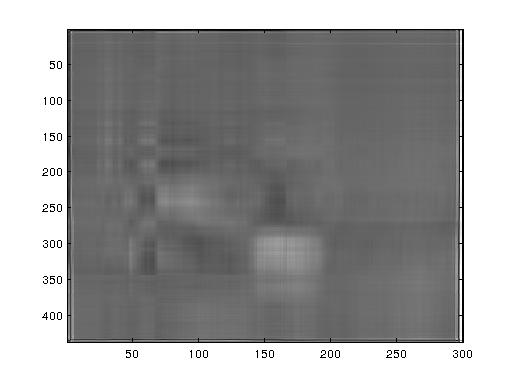
\includegraphics[scale=0.75]{d5}\protect\caption{Durer rank 5 approximation}
\end{figure}
\begin{figure}[H]
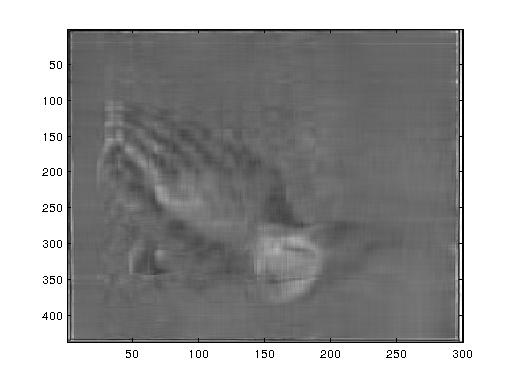
\includegraphics[scale=0.75]{d15}\protect\caption{Durer rank 15 approximation}
\end{figure}
\begin{figure}[H]
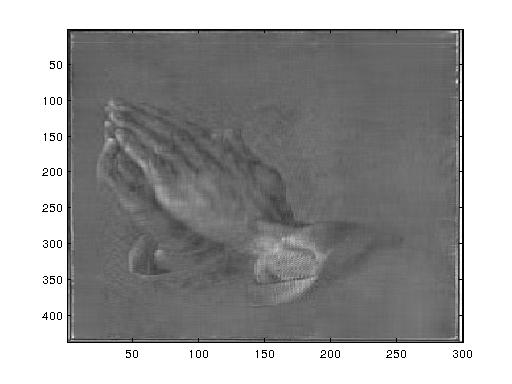
\includegraphics[scale=0.75]{d30}\protect\caption{Durer rank 30 approximation}
\end{figure}
\begin{figure}[H]
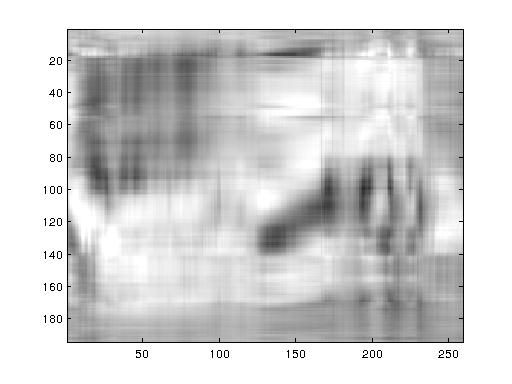
\includegraphics[scale=0.75]{e5}\protect\caption{Escher rank 5 approximation}
\end{figure}
\begin{figure}[H]
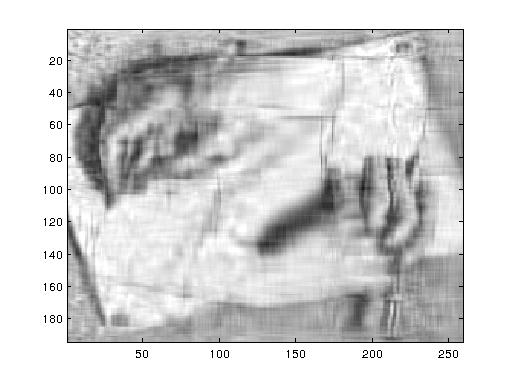
\includegraphics[scale=0.75]{e15}\protect\caption{Escher rank 15 approximation}
\end{figure}
\begin{figure}[H]
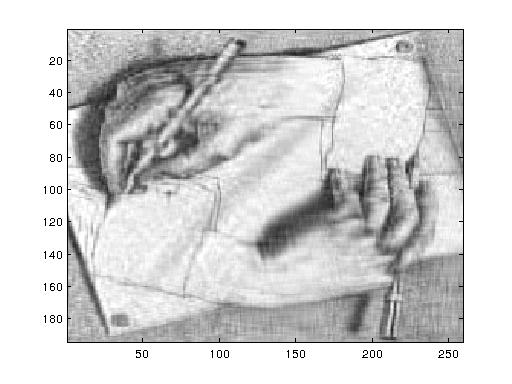
\includegraphics[scale=0.75]{e30}\protect\caption{Escher rank 30 approximation}
\end{figure}

\item [6.1]Claim: $U,V\in\mathbb{R}$ be open. Then $U\times V$ is open
in $\mathbb{R}^{2}$.

\begin{proof}
Take $\mathbf{x}=\left(x_{1},x_{2}\right)\in U\times V$. We seek
and open ball around $\mathbf{x}$ contained in $U\times V$. Let
$U,V\in\mathbb{R}$ be open. Then $x_{1}\in U$ and there exists an
openball centered on $x_{1}$such that $B_{x_{1}}\left(\epsilon_{1}\right)\subset U$.
Similarly there exists an openball centered on $x_{1}$such that $B_{x_{2}}\left(\epsilon_{2}\right)\subset V$.
Therefore $\left(x_{1},x_{2}\right)\in B_{x_{1}}\left(\epsilon_{1}\right)\times B_{x_{2}}\left(\epsilon_{2}\right)\subset U\times V$.
Take $\epsilon=\min\left\{ \epsilon_{1},\epsilon_{2}\right\} $ and
the openball centered on $\left(x_{1},x_{2}\right)$ with radius $\epsilon$
contained in $U\times V$, i.e.
\[
B_{\left(x_{1},x_{2}\right)}\left(\epsilon\right)\subset U\times V
\]

\end{proof}
\item [6.2]Claim: $\sum_{i=1}^{\infty}\frac{1}{k!}$ converges.

\begin{proof}
Note that $1/k!\leq2^{1-k}$ and 
\[
\frac{1}{2}\sum_{i=0}^{k}\frac{1}{2^{k}}=\frac{1}{2}\left(\frac{1-\left(\frac{1}{2}\right)^{k+1}}{1-\frac{1}{2}}\right)=1-\left(\frac{1}{2}\right)^{k+1}\leq1
\]
Therefore $\sum_{i=1}^{n}\frac{1}{k!}$ is monotonically increasing
and bounded above by $1$ and hence converges.
\end{proof}
\item [6.3]Claim: $\sum_{i=1}^{\infty}\frac{1}{k^{2}}$ converges.

\begin{proof}
Without loss of generality consider, for $2\leq m\leq n$ 
\begin{align*}
\left|\sum_{i=1}^{n}\frac{1}{k^{2}}-\sum_{i=1}^{m-1}\frac{1}{k^{2}}\right| & =\left|\sum_{i=m}^{n}\frac{1}{k^{2}}\right|\\
 & \leq\left|\sum_{i=m}^{n}\frac{1}{k\left(k-1\right)}\right|\\
 & =\left|-\left(\sum_{i=m}^{n}\frac{1}{k}-\frac{1}{k-1}\right)\right|\\
 & =\left|-\left(\frac{1}{n}-\frac{1}{m-1}\right)\right|=\left|\frac{1}{n}-\frac{1}{m-1}\right|\\
 & \leq\left|\frac{1}{n}\right|+\left|\frac{1}{m-1}\right|
\end{align*}
Therefore pick $N$ such that $1/N\leq\epsilon/2$ and $m\geq N+1$
then
\[
\left|\sum_{i=1}^{n}\frac{1}{k^{2}}-\sum_{i=1}^{m-1}\frac{1}{k^{2}}\right|\leq\left|\frac{1}{n}\right|+\left|\frac{1}{m-1}\right|\leq\frac{1}{N}+\frac{1}{N}\leq\epsilon
\]
Hence the sequence of partial sums is Cauchy and so the series converges.

Actually we can show that this series converges by computing its limit
explicitly. Let $f\left(x\right)=x$ be defined on $\left(-\pi,\pi\right)$.
The Fourier series expansion of $f$
\begin{align*}
f\left(x\right) & =\left(\frac{1}{2}\int_{-\pi}^{\pi}xdx\right)+\sum_{n=1}^{\infty}\left(\left(\int_{-\pi}^{\pi}x\cos\left(nx\right)dx\right)\cos\left(nx\right)+\left(\int_{-\pi}^{\pi}x\sin\left(nx\right)dx\right)\sin\left(nx\right)\right)\\
 & =\sum_{n=1}^{\infty}\left(\left(\int_{-\pi}^{\pi}x\sin\left(nx\right)dx\right)\sin\left(nx\right)\right)
\end{align*}
 by the ``oddness'' of $x\cos\left(nx\right)$ for all $n$, and
so 
\begin{align*}
f\left(x\right) & =\sum_{n=1}^{\infty}\left(\left(\frac{2}{\pi n^{2}}\sin\left(n\pi\right)-\frac{2}{n}\cos\left(n\pi\right)\right)\sin\left(nx\right)\right)\\
 & =2\sum_{n=1}^{\infty}\frac{\left(-1\right)^{n+1}}{n}\sin\left(nx\right)
\end{align*}
Then by Parseval's identity 
\[
\frac{\pi^{2}}{3}=\frac{1}{2\pi}\int_{-\pi}^{\pi}x^{2}dx=\sum_{n=-\infty,n\eqcirc0}^{\infty}\left|\frac{\left(-1\right)^{n+1}}{n}\right|^{2}=\underset{n\neq0}{\sum_{n=\infty}^{\infty}}\frac{1}{n^{2}}=2\sum_{n=1}^{\infty}\frac{1}{n^{2}}
\]
and therefore
\[
\sum_{i=1}^{\infty}\frac{1}{n^{2}}=\frac{\pi^{2}}{6}
\]
\end{proof}
\end{enumerate}

\end{document}
